% Naming convention: M_q_maxgen_scale_line-width

\documentclass[crop]{standalone}

\usepackage{tikz,tikzscale}
\usetikzlibrary{calc}

\usepackage{xifthen}


\begin{document}
  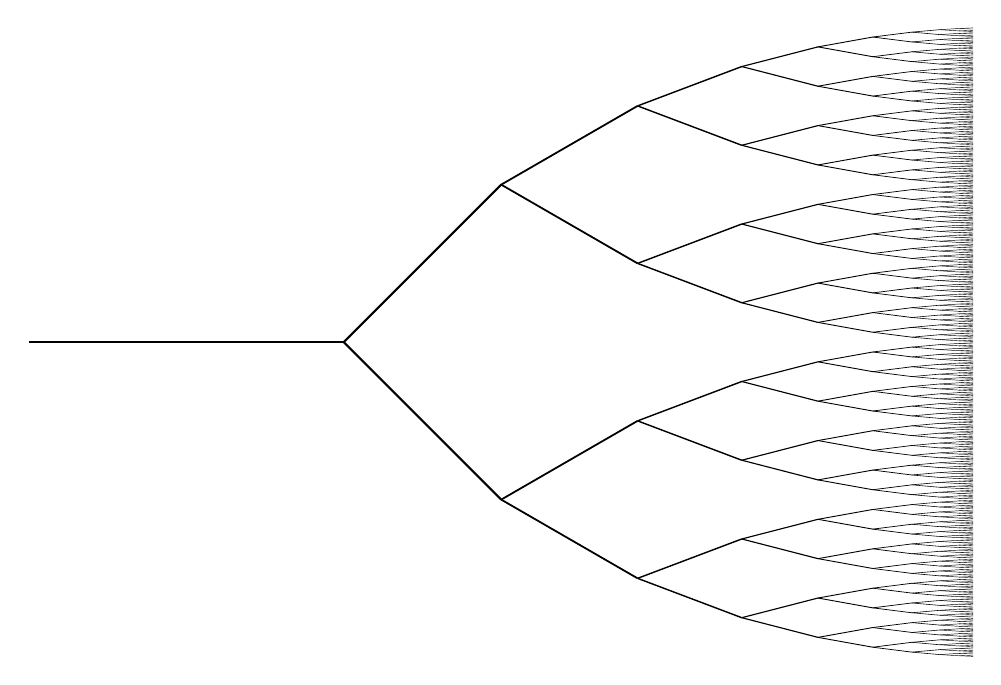
\begin{tikzpicture}[vertex/.style={draw,circle,minimum size=1.3mm,inner sep=0pt,outer sep=0pt,fill=black},scale=4]


  \def\snowflake#1#2#3{
    \newcount\gen
    \pgfmathsetmacro{\m}{#1}
    \pgfmathsetmacro{\q}{#2}
    \pgfmathsetmacro{\maxgen}{#3}
    \pgfmathsetmacro{\lw}{0.8}
    \draw[line width=\lw] (-1, 0) -- (0, 0);
    \def\doit##1##2##3##4{
      \gen=##4
      \ifnum\the\gen<\maxgen {
        \advance\gen by 1
        \pgfmathsetmacro{\prevx}{##1}
        \pgfmathsetmacro{\prevy}{##2}
        \pgfmathsetmacro{\dy}{##3}
        \foreach \i in {-1,1} {
          \pgfmathsetmacro{\angle}{asin(\dy/(2*\q^\gen)}
          \pgfmathsetmacro{\nextx}{\prevx + \q^\gen*cos(\i*\angle)}
          \pgfmathsetmacro{\nexty}{\prevy + \q^\gen*sin(\i*\angle)}
          \draw[line width=\lw^\gen] ({\prevx}, {\prevy}) -- ({\nextx}, {\nexty});
          \pgfmathsetmacro{\nextdy}{\nexty-\prevy}
          \doit{\nextx}{\nexty}{\nextdy}{\the\gen}
        }
      }
      \fi
    }
    \doit{0}{0}{1}{0}
  }

  \snowflake{2}{sqrt(1/2)}{9}

  \end{tikzpicture}
\end{document}
